\chapter{String Regeneration Applied to Machine Translation}
\label{chap:gyroTrans}

% TODO harmonize notation 1st pass vs. first pass first-pass
% TODO remove mismatch between 34.92 and 34.96
% TODO add row numbers to all tables
% TODO replace 1-best by 1st-best where appropriate
% TODO make short running title

In the previous chapter, we
have demonstrated the effectiveness of phrase-based
translation techniques for the string regeneration task.
In this chapter, we apply these techniques to the output
of a machine translation system.

Our motivation is the general motivation for the rescoring paradigm.
Instead of allowing any kind of reordering in first pass
decoding, we first create a search space of relatively high
quality, then we relax reordering constraints.
We will show that using our string regeneration decoder,
we are able to match the quality of our translation
system. In some instances, we show very slight gains in
performance.

In \autoref{sec:gyroTransExpSetting}, we describe
our machine translation baseline system.
In \autoref{sec:gyroTransBaseline}, we describe
our string regeneration baseline, both with and without
future cost estimates. Because the regeneration baseline
degrades performance with respect to the translation
baseline, we carry out error analysis
in \autoref{sec:gyroTransErrorAnalysis}.
In \autoref{sec:gyroTransBiasedLm} and
in \autoref{sec:gyroTransSysComb}, we show two ways of incorporating
information from the translation system in order to match
the translation system quality; in some instances,
we obtain very slight improvements.
Finally, in \autoref{sec:gyroTransConfidenceRegions} (TODO section being written
because still waiting for results), we show
how to exploit confidence regions in order to segment
the translation output in a meaningful way before running
our regeneration decoder.

\section{Experimental Setting}
\label{sec:gyroTransExpSetting}

In this section, we briefly summarize the machine translation
system used as a baseline for our string regeneration rescoring
experiments.

%chinese wc: 9221421 202984470 764720109
%english wc: 9221421 218009927 766246848

The Cambridge University Engineering Department participated in the
NIST 2012 translation
competition.\footnote{\url{http://www.nist.gov/itl/iad/mig/openmt12.cfm}}
We use all the Chinese-English parallel data
available for the constrained track. Parallel data consists
of 9.2M sentence pairs, 203M tokens on the Chinese side and
218M tokens on the English side, after preprocessing.
Parallel data is aligned using a word-to-phrase
HMM model with the MTTK
toolkit~\citep{deng-and-byrne:2008:ASLP}. % TODO maybe specify length
The final alignments are obtained by taking
the union of alignments obtained
in both source-to-target and target-to-source directions.
A synchronous context-free grammar is extracted from
the alignments using the infrastructure described
in \autoref{sec:rulextractMapReduce}.

We build a first-pass language model with the target side
of the parallel data and the AFP and Xinhua agencies of the
GigaWord~\citep{parker-graff-kong-chen-maeda:2009:LDC}. % TODO review bibtex entry
We build a modified Kneser-Ney 4-gram language model
on these three corpora. The language models built on AFP
and Xinhua are interpolated with equal weights. The
resulting language model is interpolated with the
language model built on the target side of the parallel
data with equal weights. We also build a second-pass
stupid backoff 5-gram language model for rescoring
as described in \autoref{sec:rescoring}.

We use the features described in \autoref{sec:features}
as well as 36 provenance related features. The union
strategy is employed for test set grammar filtering, as described
in (TODO ref to union strategy).

The results are reported in \autoref{tab:nist12results}:
%
\begin{table}
  \begin{center}
    \begin{tabular}{l|l|l}
      Config   & Tune & MT08 \\
      \hline
      1st Pass & 34.92 & 35.71 \\
      +5g      & 36.04 & 36.60 \\
      +lmbr    & 36.80 & 37.59 \\
    \end{tabular}
    \caption{NIST 2012 results for the CUED system.}
    \label{tab:nist12results}
  \end{center}
\end{table}

%TODO describe Tune and MT08

\section{NgramGen Baseline}
\label{sec:gyroTransBaseline}

% TODO check NgramGen naming

We now describe the baseline for NgramGen.
We extract the 10-best hypotheses from the lattices
obtained by first-pass translation decoding. Thus we obtain
10 sets of bag-of-words. We then run our regeneration decoder
NgramGen on each
set of bag-of-words separately.
We use the following settings for the regeneration decoder:
%
\begin{itemize}
  \item $n$-best pruning of 1000.
  \item chopping according to punctuation (comma and semi-colon) and a maximum chunk
    length of 11.
  \item future cost estimated with a unigram language model.
\end{itemize}
%
\autoref{tab:gyroMTbaseline} shows the baseline results.
%
\begin{table}
  \begin{center}
    \begin{tabular}{l|l|l|l}
      Config & Tune BLEU & Tune Oracle BLEU & MT08 BLEU \\
      \hline
      MT Baseline & 34.96 & 56.12 & 35.71 \\
      \hline
      1st-best & 33.37 & 39.14 & 32.78 \\
      2nd-best & 33.16 & 38.93 & 32.77 \\
      3rd-best & 33.14 & 38.84 & 32.54 \\
      4th-best & 33.13 & 38.80 & 32.35 \\
      5th-best & 33.20 & 38.95 & 32.12 \\
      6th-best & 33.08 & 38.74 & 32.33 \\
      7th-best & 33.19 & 39.00 & 32.16 \\
      8th-best & 32.98 & 38.79 & 32.11 \\
      9th-best & 32.71 & 38.59 & 32.11 \\
      10th-best & 33.05 & 38.81 & 32.50 \\
      union & 32.85 & 43.96 & 32.11 \\
    \end{tabular}
  \end{center}
  \caption{NgramGen baseline.}
  \label{tab:gyroMTbaseline}
\end{table}
%
Since we are only using the language model feature for the regeneration
decoder, we can observe an important drop in performance with respect
to the machine translation baseline. The union configuration means
that we form the union of the lattices obtained from NgramGen on
the 1st-best MT hypothesis up to the 10th-best MT hypothesis.
It is interesting to observe that
the oracle hypothesis obtained from the union configuration is
around 10 BLEU points above the MT baseline. This indicates that
there is a possible reordering of the 10-best hypotheses obtained by
the translation decoder that improves translation quality.

We rerun our baseline, this time including future cost estimates
in decoding. We obtain slight gains with respect to the regeneration
baseline, but gains are very small, compared to the ones obtained
when regenerating a well-formed English sentence as in \autoref{sec:gytoFutureCost}.
%
\begin{table}
  \begin{center}
    \begin{tabular}{l|l|l|l}
      Config & Tune BLEU & Tune Oracle BLEU & MT08 BLEU \\
      \hline
      MT Baseline & 34.96 & 56.12 & 35.71 \\
      \hline
      1 & 33.40 & 39.18 & 32.79 \\
      2 & 33.22 & 39.02 & 32.77 \\
      3 & 33.17 & 38.91 & 32.55 \\
      4 & 33.16 & 38.87 & 32.39 \\
      5 & 33.28 & 39.00 & 32.17 \\
      6 & 33.12 & 38.81 & 32.40 \\
      7 & 33.24 & 39.05 & 32.18 \\
      8 & 33.04 & 38.84 & 32.14 \\
      9 & 32.75 & 38.65 & 32.11 \\
      10 & 33.11 & 38.88 & 32.55 \\
      union & 32.90 & 44.00 & 32.18 \\
    \end{tabular}
  \end{center}
  \caption{Effect of using future cost estimates.}
\end{table}
%
In the next section, we will analyze the drop in performance
when running our regeneration decoder on the output
of the translation decoder.

\section{Error Analysis}
\label{sec:gyroTransErrorAnalysis}

% TODO maybe compare lm costs

We have observed that simply reordering the $n$-best output
of the translation decoder with our technique gives a drop
in performance. We wish to examine how often the MT
hypothesis is not regenerated and at what point in decoding
it gets lost.

When reordering the first-best MT hypothesis on the Tune set,
the MT hypothesis is present in the regeneration lattice
92.3\% of the time. In contrast, the MT 1-best is regenerated
only 43.6\% of the time. When including future cost, the MT
hypothesis is present in the regeneration lattice
more often: 95.3\% of the time while the MT hypothesis is regenerated
with the same frequency: 43.6\% of the time.
\autoref{fig:whenLostInput} shows at what point the MT hypothesis is lost
when running the generation decoder. The left hand side plot shows that
that the MT hypothesis can be lost quite early in the process, as early as
when 20\% of the size of the input bag of word has been covered. The right
hand side plot shows that using future cost estimates alleviate this problem
but not entirely.
%
\begin{figure}
\begin{center}
\begin{minipage}{.45\textwidth}
  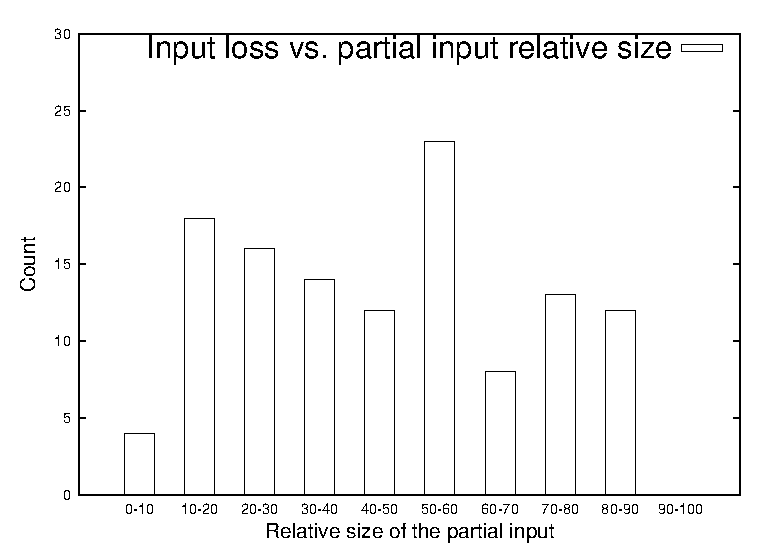
\includegraphics[scale = 0.6]{figures/whenLostInput/Tune.text.nw.v3x08.1stpass.10best.exp.allrules.mmap.nbest1000.1.whenlostinput.eps}
\end{minipage} 
\hfill
\begin{minipage}{.45\textwidth}
  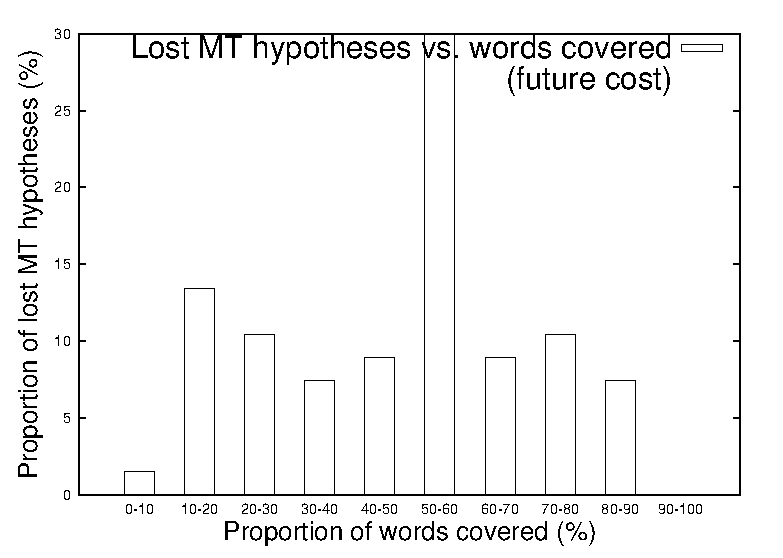
\includegraphics[scale = 0.6]{figures/whenLostInput/Tune.text.nw.v3x08.1stpass.10best.exp.allrules.mmap.nbest1000.1.futurecost.whenlostinput.eps}
\end{minipage}
\caption{Analysis of when the MT hypothesis is lost. The x-axis represents bins of 10\% for the relative size of the input bag-of-word.
The y-axis is simply the count of instances. Future cost estimates are used in decoding for the right hand side figure.}
\label{fig:whenLostInput}
\end{center}
\end{figure}
%
In the next two sections, we will describe two ways of incorporating
information from the translation system in order to at least
match the quality of the translation system.

\section{Regenerate the input with biased lm}
\label{sec:gyroTransBiasedLm}

We have shown in the previous section, that the MT hypothesis, which
we know to be of relatively high quality, is often not regenerated.
In this section, we describe a first solution to remedy this issue.

Our solution is to bias the language model towards the MT hypothesis.
In order to do this, we compute $n$-gram posteriors from the
1st-pass translation lattices~\citep{blackwood:2010:PHD}.
We then convert the posteriors
to integer counts and estimate a
Good-Turing~\citep{good:1953:biometrika,chen-goodman:1998:harvard} smoothed 4-gram
language model from these counts.
We then interpolate this language model with the original language model with
various interpolation parameters.
We obtain the results in \autoref{tab:gyroBiasedLm}.
%
\begin{table}
  \begin{center}
    \begin{tabular}{l|l}
      Config      & Tune BLEU \\
      \hline
      MT Baseline (1st pass) & 34.96 \\
      \hline
      1st-best      & 33.37 \\
      \hline
      1st-best 0.4  & 34.96 \\
      1st-best 0.5  & 34.96 \\
      1st-best 0.6  & 34.96 \\
      1st-best 0.7  & 34.97 \\
      1st-best 0.8  & 34.94 \\
      1st-best 0.9  & 34.90 \\
      1st-best 0.95 & 34.81 \\
      1st-best 0.99 & 34.11 \\
    \end{tabular}
    \caption{Regenerating the MT 1st-best with a biased language model.
      The interpolation parameter is the interpolation weight of the
      original language model.}
    \label{tab:gyroBiasedLm}
  \end{center}
\end{table}
%
We can see that we are able to obtain hypotheses that have
the same quality as the MT hypotheses, and for an interpolation
weight of 0.7, we obtain a very slight improvement on the tuning
set.
We obtain very similar results when we include future cost estimates.
We use the best interpolation weight of 0.7 to run
our regeneration decoder on the test set MT08 and obtain results
in \autoref{tab:gyroBiasedLmTest}.
We obtain slight gains in terms of BLEU score on the MT08 test
using this technique.
%
\begin{table}
  \begin{center}
    \begin{tabular}{l|l|l}
      Config & Tune BLEU & MT08 BLEU \\
      \hline
      MT Baseline (1st pass) & 34.96 & 35.71 \\
      \hline
      1st-best Interpolation 0.7 & 34.97 & 35.75 \\
      1st-best Interpolation 0.7 Future Cost & 34.96 & 35.75 \\
    \end{tabular}
    \caption{Effect of using a language model biased towards
    translation posteriors.}
    \label{tab:gyroBiasedLmTest}
  \end{center}
\end{table}

% TODO maybe redo with less pruning ??

%biased lm union
%\begin{table}
%  \begin{center}
%    \begin{tabular}{l|l|l}
%      Config      & BLEU & Oracle BLEU \\
%      MT Baseline & 34.96 & 56.12 \\
%      union       & 0.3285 & 43.96 \\
%      union 0.4   & TODO
%      union 0.5
%      union 0.6
%      union 0.7
%      union 0.8
%      union 0.9
%      union 0.95
%      union 0.99
%    \end{tabular}
%    \caption{TODO caption}
%  \end{center}
%\end{table}

%biased lm future cost
%\begin{table}
%  \begin{center}
%    \begin{tabular}{l|l|l|l}
%      Config      & BLEU & Oracle BLEU & MT08 \\
%      MT Baseline & 34.96 & 56.12 & 35.71  \\
%      1-best      & 33.40 & 39.18 & 32.79 \\
%      1-best 0.4  & 34.95 & & \\
%      1-best 0.5  & 34.96 &  & \\
%      1-best 0.6  & 34.96 &  & \\
%      1-best 0.7  & 34.96 & & 0.3575 YAY! \\
%      1-best 0.8  & 34.94 & & \\
%      1-best 0.9  & 34.90 & & \\
%      1-best 0.95 & 34.81 & & \\
%      1-best 0.99 & 34.13 & & \\
%    \end{tabular}
%    \caption{TODO caption}
%  \end{center}
%\end{table}

\section{Hypothesis Combination}
\label{sec:gyroTransSysComb}

In the previous section, we have described one way
to obtain hypotheses of comparable quality to the
MT hypotheses. In this section, we present some
hypothesis combination results.
Our hypothesis combination technique
is described in \autoref{sec:lmbr} and is
based on lattice Minimum Bayes' Risk
decoding~\citep{blackwood:2010:PHD}.

Results are presented in \autoref{tab:gyroTransSysComb}.
We can observe that using the union of lattices produced
by NgramGen is beneficial for hypothesis combination.
Using the biased language model described in the
previous section, we are able to match and obtain
a very slight gain over the LMBR rescored translation
hypotheses.
%TODO add row numbers
% TODO describe how gyro is 5g rescored before combination
\begin{table}
  \begin{center}
    \begin{tabular}{l|l|l}
      Config & Tune BLEU & MT08 BLEU \\
      \hline
      MT Baseline (LMBR) & 36.80 & 37.59 \\
      \hline
      NgramGen 1-best Baseline &  36.81 & 37.29 \\
      NgramGen union Baseline & 36.81 & 37.50 \\
      \hline
      NgramGen 1-best Baseline Future Cost & 36.82 & 37.45 \\
      NgramGen union Baseline Future Cost & 36.81 & 37.50 \\
      \hline
      NgramGen 1-best Interp 0.7 & 36.82 & 37.39 \\
      NgramGen union Interp 0.7 & 36.78 & 37.59 \\
      \hline
      NgramGen 1-best Interp 0.7 Future Cost & 36.81 & 37.39 \\
      NgramGen union Interp 0.7 Future Cost & 36.77 & 37.60 \\
    \end{tabular}
    \caption{Hypothesis combination between the output of the translation
    decoder and the output of the regeneration decoder.}
    \label{tab:gyroTransSysComb}
  \end{center}
\end{table}

%\section{Exploiting Confidence Regions}
%\label{sec:gyroTransConfidenceRegions}

%\begin{table}
%  \begin{center}
%    \begin{tabular}{l|l|l}
%      Config & Tune & MT08 \\
%      MT Baseline & 34.96 & 35.71 \\
%      Gyro Baseline & 33.37 & 32.78 \\
%      beta 0.3 & 32.93 &  \\
%      beta 0.4 & 32.94 & \\
%    \end{tabular}
%    \caption{TODO caption}
%  \end{center}
%\end{table}

\section{Conclusion}

In this chapter, we have shown how to apply our regeneration
decoder to the output of a translation system in a 10-best hypothesis
rescoring setting. Because the regeneration decoder only uses
a language model as single feature and throws away ordering
information obtained from the translation system, by simply
running NgramGen on the output of the translation system, translation
performance is degraded.

We have shown two possible ways of integrating the information from the
translation system into the regeneration system in order to match
and slightly outperform the translation quality obtained by the
translation system. The first solution is to bias the language
model used in regeneration towards the MT hypotheses. The second
solution simply takes advantage of well known hypothesis combination
techniques.

%\begin{itemize}
%  \item Experiment with bag of word made of 1-best translation. Show oracle scores. OK
%  \item Experiment with bag of word made of 1-best to 10-best translation. Show oracle scores. OK
%  \item Error analysis: show how often at what stage the input is lost. Conclusion: the
%    decoder needs to be biased towards the input. OK when lost input OK
%  \item Experiments on biasing the decoder towards the input: build language models
%    based on the MT output or based on the MT posteriors. OK
%  \item System combination experiments. OK
%  \item MAYBE: Syntactic n-grams experiments: use the syntactic n-grams to enrich the
%    bag of words and use the dependencies in conjunction with the dependency LM.
%  \item Use gyro together with confidence regions: the confidence regions can be used
%    for chopping and constraints. RUNS
%  \item MAYBE: Use gyro together with position specific posteriors (TBA).
%\end{itemize}
